\section{Chapter 1: Learning General-purpose Neural Field Over the Earth}
\label{sec:sat2cap}
Dhakal, Aayush, et al. ``RANGE: Retrieval Augmented Neural Fields for Multi-Resolution Geo-Embeddings." \textit{Proceedings of the Computer Vision and Pattern Recognition Conference. 2025.}
\subsection{Overview}
Our primary objective is to learn a neural field, $R=F_\theta(lat, lon)$, where $R$ is a powerful general-purpose representation. After learning this neural field, we aim to utilize $R$ to solve various geospatial downstream tasks more effectively.  

Geolocation is a vital modality that possesses highly unique characteristics, such as low dimensions and circular input. In this chapter, we will explore methods for learning effective representations for geolocation. Previous work~\cite{russwurm2023geographic} has shown that using location directly (represented as two floating point numbers of latitude and longitude) as an input to a machine learning model yields poor performance. Therefore, several works have attempted to find better ways to represent location data. A common approach used by state-of-the-art models~\cite{vivanco2024geoclip,mai2023csp,klemmer2023satclip} involves learning visual cues associated with a given geolocation. Two recent state-of-the-art models, GeoCLIP~\cite{vivanco2024geoclip} and SatCLIP~\cite{klemmer2023satclip}, use contrastive training to align geo-embeddings with co-located images; the former aligns them with ground-level images while the latter aligns them with satellite images. In this work, we argue that the current approaches to learning geo-embeddings using images, while powerful, still fail to preserve all the relevant visual information. To address this issue, we propose a retrieval-augmented
strategy that approximates the unique visual information
present in a location. We formally define the problem in Section~\ref{sec:multi-view}, and propose our solution in Section~\ref{sec:range-method}
 \begin{figure*}[!t]
\begin{center}
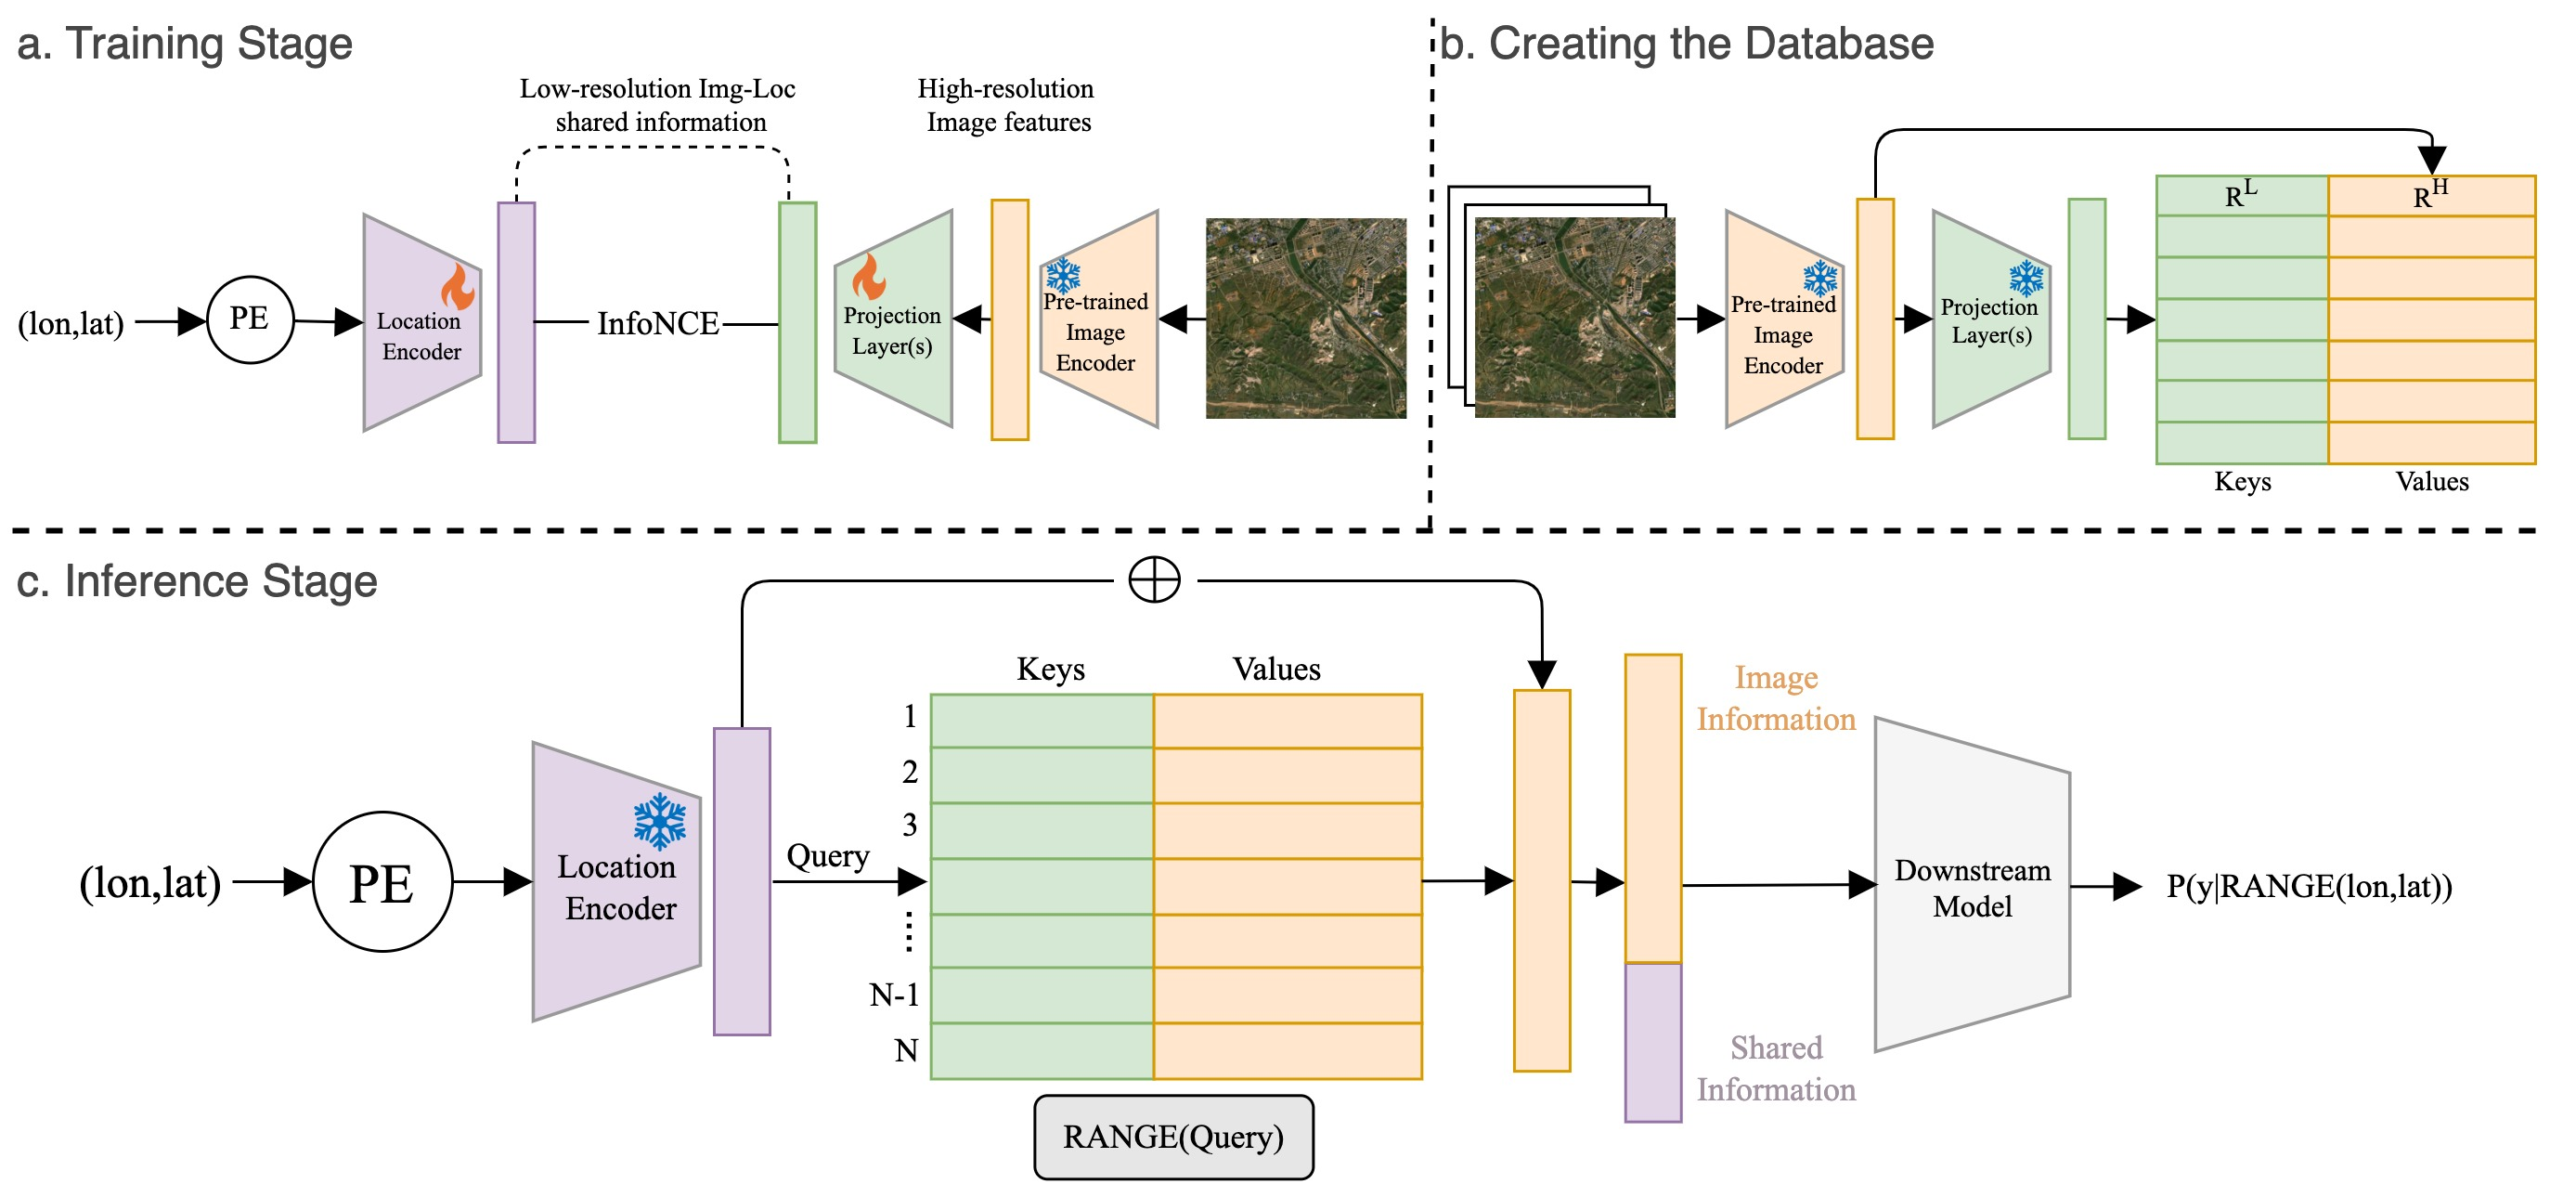
\includegraphics[width=\linewidth, scale=0.3]{proposal/images/framework_cam.jpg}
\end{center}
    \caption{Framework of RANGE. (a) In the training stage, a shared embedding space is learned between locations and images. (b) We create a database of low-resolution and high-resolution image embeddings using the trained projection layer and a powerful pretrained image model, respectively. (c) During inference, we use a location as the query, low-resolution image embeddings as keys, and high-resolution image embeddings as values. Using our retriever function, we compute the approximate high-resolution embeddings for the query. We concatenate ($\oplus$) the approximated visual feature with our query embedding.} 
\label{fig:framework}
\end{figure*}
\subsection{Aligning Location and Image is a Multi-View Non-Redundancy Problem}
\label{sec:multi-view}
Let (L,H,T) represent location modality, image modality, and geospatial task, respectively. Models like SatCLIP and GeoCLIP align co-located images and locations by minimizing the infoNCE objective. Solving the multimodal infoNCE objective maximizes the lower bound on the mutual information, preserving the shared information within the learned representations~\cite{oord2018representation}. As such, the final learned representations of these models contain only information that is shared across both location and image. This property is useful under the multi-view redundancy assumption, which states that the information shared between the two modalities is exactly relevant to solve the underlying task~\cite{tosh2021contrastive}. However, this assumption does not hold in the location-image learning setting, as there is high unique information contained in the image modality that is useful for solving downstream tasks. Formally, we argue that location-image learning falls under the multi-view non-redundancy setting: there is \textit{unique} information in the image modality that is not shared with the location modality, and that information is relevant for solving our geospatial task T. In this case, contrastive training discards valuable task-relevant information from the image, leading to poor downstream performance~\cite{liang2023factorized}.

\subsection{Method}
\label{sec:range-method}
We consider a dataset with paired geolocations and co-located satellite images $\{g_i, s_i\}$. The goal is to learn a meaningful representation for $g_i$ by aligning it with $s_i$, which can be done by minimizing the clip objective \cite{klemmer2023satclip, vivanco2024geoclip, radford2021learning}. We have a trainable geolocation encoder $E$, a frozen pretrained image encoder $I$, and a projection layer $P$. Let $G_i = E(g_i)$ represent the location embedding, $S_i = {I(s_i)}$ represent the frozen image embedding, and $P_i = P(I(s_i))=P(S_i)$ represent the image embedding obtained from the projection layer for the i$^{th}$ sample. We minimize the objective:
%
\begin{align}
&L_{i}^{loc} = \frac{-1}{k}\sum_{i=1}^{k} \log\frac{\exp(G_i \cdot P_i / \tau)}{\sum_{j=1}^{k} \exp(G_i \cdot P_j) / \tau) } \\
&L_{i}^{img} = \frac{-1}{k}\sum_{i=1}^{k} \log\frac{\exp(G_i \cdot P_i / \tau)}{\sum_{j=1}^{k} \exp(G_j \cdot P_i) / \tau) } \\
&L_i = (L_i^{loc} + L_i^{img})/2 
\end{align}
%
The training process is shown in Figure~\ref{fig:framework}-(a). We contrastively align the geolocations and satellite images by minimizing their CLIP objective. This formulation is identical to SatCLIP~\cite{klemmer2023satclip}, so we use the pretrained SatCLIP image and location encoders for simplicity. For query location $g_i$, $S_i$ encodes the high-resolution visual features since $I$ is a powerful pre-trained image encoder. Both $P_i$ and $G_i$ encode low-resolution shared information between $g_i$ and $s_i$. The resulting geo-embedding, $G_i$, is sub-optimal as it loses unique visual information crucial for many downstream tasks. To solve this, we propose a retriever function $R_\tau$ that allows us to approximate the high-resolution information $S_i$ given $g_i$. Let $\epsilon$ denote the deviation from the true visual embedding. We can then explicitly add the approximate visual information $\hat{S_i}$ to our location embedding $G_i$:
    \begin{align}
    &R_\tau(g_i) = \hat{S_i} = S_i + \epsilon \\
    &RANGE(g_i) = \hat{S_i} \oplus G_i 
    \end{align}

\begin{table}
\centering    

% \hspace*{-1.3cm}
\resizebox{\linewidth}{!}{
\begin{tabular}{l|ccc|ccccc}
\hline
                        & Biome & EcoRegions & Country   & Temperature & Elevation & Population & Cali-Housing   \\ \hline
Direct                      & 29.1 & 0.6 & 66.9& 0.381  & 0.025  &  0.053  & 0.238      \\
Cartesian\_3D                      & 30.2 & 1.8 &66.9 & 0.362  & 0.030  &  0.162  & 0.240      \\
Wrap~\cite{Aodha_2019_ICCV}                      & 34.4 & 1.1 & 69.7& 0.861  & 0.085  &  0.328  & 0.239      \\
Theory~\cite{gaolearning}                      & 33.5 & 1.0 &72.5 & 0.849  & 0.093  &  0.330  & 0.254      \\
SphereM~\cite{mai2023sphere2vec}                      & 36.4 & 27.3 & 72.7 & 0.629  & 0.139  &  0.302  & 0.423      \\
SphereM$^{+}$~\cite{mai2023sphere2vec}                      & 58.7 & 50.1 & 76.1 & 0.886  & 0.294  &  0.421  & 0.543      \\
SphereC~\cite{mai2023sphere2vec}                     & 36.3 & 52.9 & 72.9 & 0.461  & 0.185  &  0.335  & 0.496      \\
SphereC$^+$~\cite{mai2023sphere2vec}  & 53.2 & 61.6 & 73.6 & 0.842  & 0.260  &  0.392  & \underline{0.544}      \\

\hline


CSP-INat~\cite{mai2023csp}                      & 61.1 & 57.1 & 75.9 & 0.717  & 0.388  &  0.554  & 0.462      \\
CSP-FMoW~\cite{mai2023csp}                    & 61.4 & 58.0 & 81.3& 0.865  & 0.399  &  0.580  & 0.541      \\
SINR~\cite{cole2023spatial}                    & 67.9 & 54.9 & 88.3 & \textbf{0.942}  & 0.644  & 0.726 & 0.420      \\
GeoCLIP~\cite{vivanco2024geoclip}                & \underline{70.2} & 71.6 & 81.3 & 0.916  &  0.604  &  0.698  & \textbf{0.708}      \\
SatCLIP~\cite{klemmer2023satclip}  & 68.9 & 69.3 & 82.8 & 0.825       & 0.666     & 0.684 & 0.400   \\ \hline


RANGE  & \textbf{83.3} & \textbf{75.7} & \underline{93.7} &0.895 & \underline{0.844} & \underline{0.799} & 0.422  \\ 


RANGE$^+$                      & \textbf{83.3} & \underline{75.3} & \textbf{94.7} &\underline{0.931} & \textbf{0.851} & \textbf{0.811} & 0.336 &    \\ 
\end{tabular}
}
\caption{Our model shows improvements over a variety of tasks compared to state-of-the-art models. The first 3 columns are classification tasks with accuracy metrics and the last 4 columns are regression tasks with R$^2$ metric. We show improvements with significant margins across many of the tasks. Our model underperforms in the Cali-housing dataset. We further analyze this behavior in our discussions.}
\label{table:main}
\end{table}

\subsubsection{Retrieval Augmented Neural Fields}
\noindent \textbf{Creating the Retrieval Database: }Once the contrastive training is done, we create a retrieval database as shown in Figure~\ref{fig:framework}-(b). We take $\{g_i, s_i\}$ sampled uniformly across the globe using the SatCLIP~\cite{klemmer2023satclip} dataset. For every location $g_i$ in our data, we compute: a) the shared-information image embedding $R_i{^L}=P(I(s_i))$, and b) the high-resolution image embedding $R_i{^H}=\bar{I}(s_i))$; we refer to these sets of embeddings as low-resolution embeddings and high-resolution embeddings, respectively, in the rest of the paper. In practice, $\bar{I}$ can differ from $I$; the only condition is that $\bar{I}$ is a pretrained image feature extractor. For our purposes, we use SatMAE~\cite{cong2022satmae} as $\bar{I}$. 
\\
\\
\noindent \textbf{Retriever Function: }
Let $R^L=\{R_{1}^L, R_{2}^L,...R_{N}^L\}$, and $R^H=\{R_{1}^H, R_{2}^H,...R_{N}^H\}$ represent the set of all low-resolution and high-resolution image embeddings in our database. After creating the database, we need a method to sample appropriate high-resolution image information for a query location. Naively, we can set this as a lookup operation, where $G_i$ is the query, $R^L$ is the set of all keys, and $R^H$ is the set of all values. We have a function $sim(G_i, R_{j}^{L})$, which gives the alignment scores between i and j. In our setting, this similarity function is a simple cosine similarity. For a query $G_i$, we find $R_{j}^{L}$ with the highest alignment score and return the key $R_{j}^{H}$. 
In practice, $R_{j}^{H}$ is noisy. The semantically closest image in the database can contain additional information that is irrelevant to the location. Therefore, naively adding $R_{j}^{H}$ has the potential of introducing incorrect information to our geo-embeddings. 



We instead use a soft selection criteria. First, we compute the query's alignment score with each key in the database using cosine similarity. We use a softmax function to convert the alignment scores to probabilities. We also use a temperature parameter $\tau$ to slightly reshape the probability distribution; $\tau$ is extremely robust as it does not need to be fine-tuned for different tasks or for databases with different distributions. We use the resulting probabilities to compute a weighted average across all values, i.e., high-resolution image embeddings in the database. The resulting embedding is an approximation of $S_i$, where the information contributed by each image is weighted by its alignment score with the query. We concatenate this approximate high-resolution image embedding with our original location embedding $G_i$ to obtain the multi-resolution RANGE embedding $RANGE_i$. A high-level view of this process is shown in Figure~\ref{fig:framework}-(c). 

\begin{equation}
    RANGE_i = R_{\tau}(G_i) \oplus G_i 
= \frac{1}{N}\sum_{k=1}^{N}{\frac{e^{sim(G_i,R_{k}^L)/\tau}}
{\sum_{j=1}^{N}{e^{sim(G_i,R_{j}^L)/\tau}}}} * R_{k}^H \oplus G_i
\end{equation}
\noindent $\text{, where}\ G_i\in \mathbb{R}^M,\ R_{k}^L \in \mathbb{R}^M,\ R_{k}^H \in \mathbb{R}^{N}.$
%
\\
\\
\noindent \textbf{Adding smoothness constraints: }We also propose another version of our model called $RANGE^+$. Here, we additionally use geodesic similarity to approximate the visual features of the location. We convert our query location to 3D cartesian coordinates and use angular distance to find the spatially closest image in the database. This spatial retrieval allows us to impose spatial smoothness on our embeddings since locations close to each other are forced to have similar retrieval, irrespective of the semantics.  The spatially retrieved embedding is added to the semantically retrieved embedding and weighted using a $\beta$ parameter, which controls the level of spatial smoothness enforced on the $RANGE$ embeddings. Let $g{_i}^{3D}$ be the query location, $l$ be the set of all database locations in 3D cartesian coordinates, and $sim(g{_i}^{3D}, l_k)$ be their angular similarity:   
\begin{multline}
\label{eq:rangep}
RANGE^+_{i} = \frac{1}{N}(\beta*\sum_{k=1}^{N}{\frac{e^{sim(G_i,R_{k}^L)/\tau_{1}}}{\sum_{j=1}^{N}{e^{sim(G_i,R_{j}^L)/\tau_{1}}}}} * R_{k}^H+ \\ 
     (1-\beta)\sum_{k=1}^{N}{\frac{e^{sim(g{_i}^{3D},l_{k})/\tau_{2}}}{\sum_{j=1}^{N}{e^{sim(g{_i}^{3D},l_{j})/\tau_{2}}}}} * R_{k}^H
     )\oplus G_i \\
\end{multline}
$\text{, where } G_i \in \mathbb{R}^M, \ g{_i}^{3D} \in \mathbb{R}^3, \ l_k \in \mathbb{R}^3$
\begin{table}[]
\centering
\begin{tabular}{l|c|ccccc}
\textbf{} & $\beta$ & \begin{tabular}[c]{@{}c@{}}100\\ \footnotesize 19.21$^\circ$\end{tabular} & \begin{tabular}[c]{@{}c@{}}500\\ \footnotesize 8.72$^\circ$\end{tabular} & \begin{tabular}[c]{@{}c@{}}1000\\ \footnotesize 6.11$^\circ$\end{tabular} & \begin{tabular}[c]{@{}c@{}}1500\\ \footnotesize 5.06$^\circ$\end{tabular} & \begin{tabular}[c]{@{}c@{}}2000\\ \footnotesize 4.34$^\circ$\end{tabular} \\ \hline

SatCLIP &  & 36.0 & 26.4 & 25.5 & 25.5 & 21.7 \\
GeoCLIP &  & 64.1 & 22.8 & 15.7 & 14.4 & 13.8 \\
CSP-INat &  & 44.9 & 27.1 & 24.0 & 21.9 & 18.5 \\
CSP &  & 67.8 & 33.8 & 26.8 & 23.9 & 21.1 \\
SINR &  & 87.6 & 58.4 & 34.3 & 22.6 & 19.0 \\
\hline
 & 0       & \textbf{94.0}                                                                            & \textbf{73.2}                                                                           & 50.0                                                                                     & 43.1                                                                                     & 37.8                                                                                     \\
          & 0.25    & \underline{93.3}                                                                               & \underline{72.6}                                                                              & \underline{55.8}                                                                               & 50.7                                                                                     & 45.3                                                                                     \\
   RANGE$^+$       & 0.5     & 92.3                                                                                     & 70.0                                                                                    & \textbf{56.4}                                                                            & \textbf{52.3}                                                                            & \textbf{47.2}                                                                            \\
          & 0.75    & 89.4                                                                                     & 65.1                                                                                    & 54.5                                                                                     & \underline {50.6}                                                                               & \underline {46.3}                                                                               \\
          & 1       & 65.7                                                                                     & 53.6                                                                                    & 50.5                                                                                     & 46.6                                                                                     & 42.6                                                                                    
\end{tabular}
\caption{We quantitatively show that controlling the beta parameter allows us to generate optimal embeddings depending on the resolution of the task. We evaluate on the checkerboard task~\cite{russwurm2023geographic} and change the number of grid cells in the Fibonacci lattice to simulate tasks with different spatial resolutions. Lower $\beta$ yields better embeddings for low-resolution tasks, whereas higher $\beta$ yields better embeddings for high-resolution tasks. We see that we outperform all the baselines across all spatial resolutions.}
\label{table:beta}

\end{table}
\subsection{Results}
\subsubsection{Quantitative Evaluation on Downstream Tasks}
We evaluate the efficacy of RANGE and RANGE$^+$ embeddings on a wide variety of downstream applications. We choose 3 classification tasks (biome, ecoregion, and country classification) and 4 regression tasks (population density estimation, temperature, elevation, and housing price prediction) for this experiment, as used by prior work~\cite{klemmer2023satclip}. We compare our method with SoTA parametric~\cite{klemmer2023satclip, vivanco2024geoclip, cole2023spatial, mai2023csp, mai2023sphere2vec} and non-parametric~\cite{Aodha_2019_ICCV,gaolearning} representations. The results of this experiment are shown in Table~\ref{table:main}. The results show that our method outperforms all state-of-the-art models in the classification tasks with significant margins. Among the regression tasks, we achieve SoTA performance for elevation and population density prediction with significant gains and narrowly come second in the air temperature prediction task. Furthermore, RANGE$^+$, on average, outperforms RANGE by a small margin, which can be attributed to the spatial smoothness constraint.

\begin{figure*}[!t]
\begin{center}
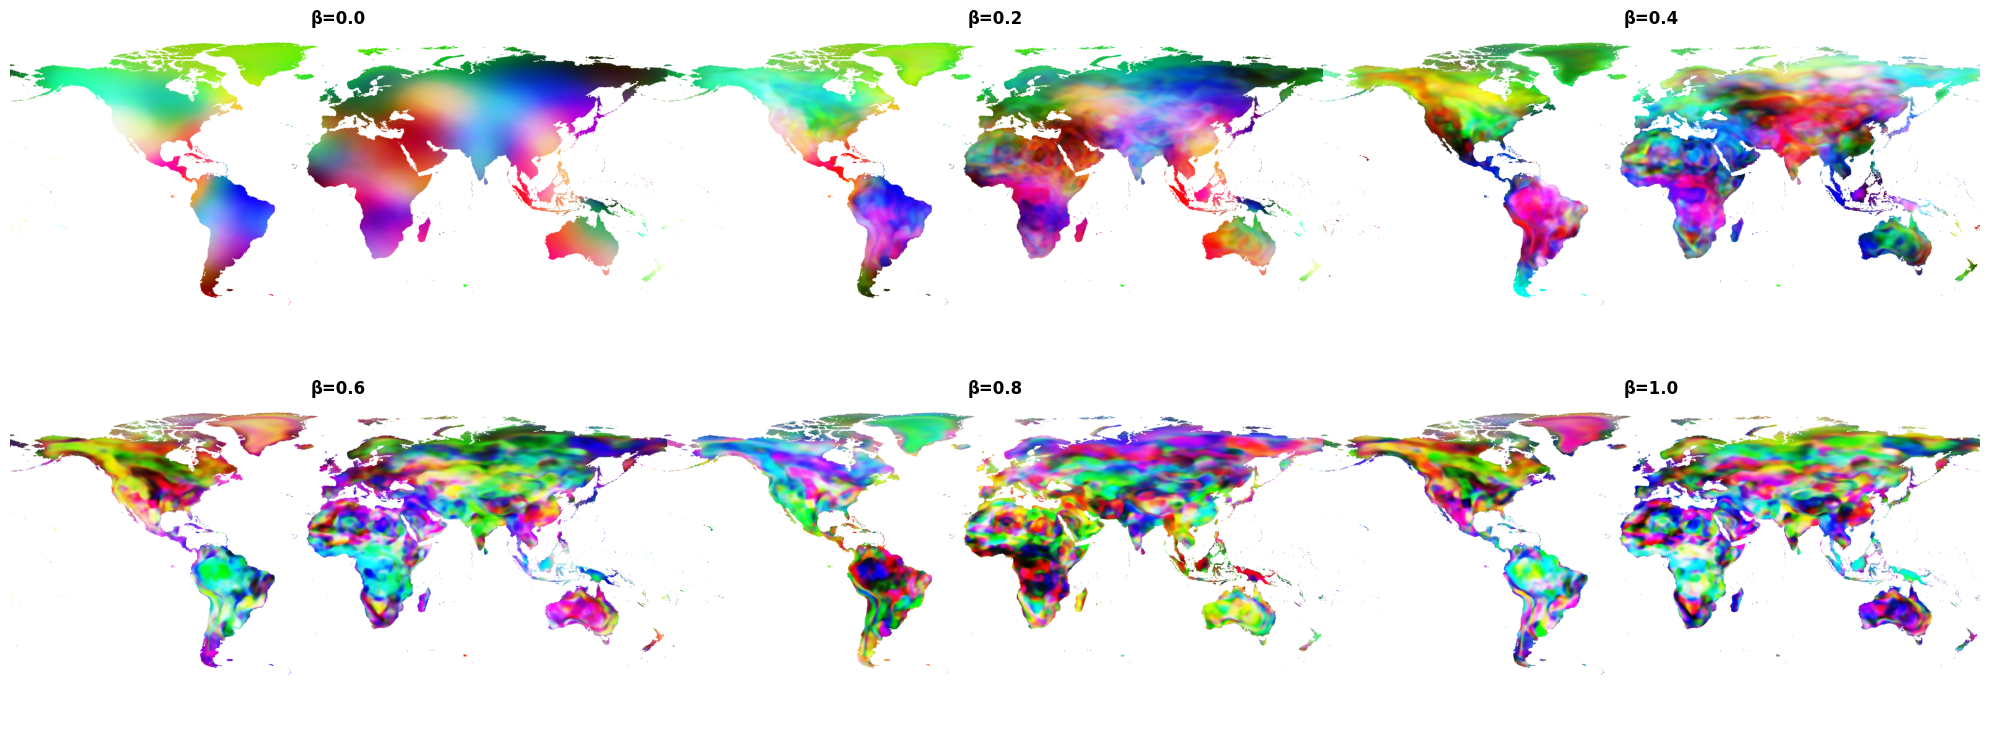
\includegraphics[width=\linewidth, scale=0.3]{proposal/images/beta_interpolation_2.png}
\end{center}
   \caption{Interpolating the $\beta$ parameter in RANGE$^+$ allows us to control the spatial smoothness of our embeddings. The results show that RANGE$^+$ can be used to generate neural fields of geo-embeddings at multiple frequencies.} 
\label{fig:beta}
\end{figure*}

\subsubsection{Understanding the Impact of $\beta$ parameter}
We attempt to understand the impact of the $\beta$ parameter in equation~\eqref{eq:rangep}. First, we perform a quantitative evaluation of varying $\beta$. Our results in Table~\ref{table:beta} show that a lower beta is optimal for low-resolution tasks, whereas a higher beta is usually better for high-resolution tasks. We also compute the ICA of the embeddings at different $\beta$ and plot them over the map of the world to qualitatively assess the differences. The results in Figure~\ref{fig:beta} show that
RANGE+ can be used to generate neural fields of geo-embeddings at multiple frequencies. 

\subsection{Proposed Direction}
We showed the utility of RANGE embeddings across a large number of downstream tasks such as population density estimation, biome prediction, fine-grained species classification etc. However, all our evaluations were limited to discriminative tasks. We will work towards understanding the utility of our general purpose neural field for solving generative tasks. Specifically, we will use RANGE embeddings to improve existing geospatial generative models. Geospatial generative models try to generate realistic looking satellite images. Our RANGE embeddings contain high-resolution information, and conditioning the generative models using these embeddings can enable improved location conditioned generation.   

\subsection{Chapter Conclusion}
In this chapter, we proposed a new framework for general purpose neural field over the earth. We showed the limitations of directly adapting generic representation learning methods for geospatial data. Specifically, we showed that using contrastive training for geolocation representation learning violates assumptions of multi-view redundancy, resulting in sub-optimal representations. We proposed a retrieval-augmented strategy for estimating visual features from an auxiliary database of visual embeddings. Our approach results in significant improvements for a variety of tasks as compared to purely parametric embedding strategies with only a modest increase in storage requirements. Hence, we highlighted the importance of designing data-specific representation learning strategies and understanding the assumptions and limitations of existing approaches. 